\section{The constant: repeating the Goldbach questions}
\label{fnd:constant}

Goldbach's conjecture asks whether every even integer greater than two is a
sum of two primes.  We begin by making a real number that remembers all of
these questions.  List the primes as $p_1=2,p_2=3,p_3=5,\ldots$, and attach
the question about $2(j+1)$ to $p_j$.  Thus the prime $2$ carries the question
about $4$, the prime $3$ the question about $6$, and so on.  Write
\[
 g_j=\mathbf1_{\{2(j+1)\text{ is a sum of two primes}\}}.
\]
Putting $g_j$ only at digit position $p_j$ would hide the answers in a set
of density zero.  Instead, we repeat each answer along a whole
\emph{prime lane}: the positive integers whose least prime factor is $p_j$.

One further ingredient gives the number its internal arithmetic.  Let
$\Omega(n)$ count prime factors with multiplicity, let
$\lambda(n)=(-1)^{\Omega(n)}$, and set $\lambda(1)=1$.  For $n\ge2$ let
$\ell(n)$ be the index of its least prime factor.  Our constant is
\begin{equation}
 x_1=0,\qquad x_n=\frac{1-\lambda(n)}2g_{\ell(n)}\quad(n\ge2),
 \qquad \Gold=\sum_{n\ge1}x_n2^{-n}.
 \label{fnd:definition}
\end{equation}
Every digit is computable by a finite calculation.  In an enabled lane,
the digit is one when the number has an odd number of prime factors,
counting multiplicity.  In a disabled lane every digit is zero.
At prime positions the Liouville factor equals $-1$, so
\begin{equation}
 x_{p_j}=g_j.
 \label{fnd:prime-reading}
\end{equation}
The prime digits therefore list the Goldbach answers exactly, while the
other digits repeat those answers in a structured way.

It is useful to permit an arbitrary binary message
$g=(g_1,g_2,\ldots)$ in the same definition.  We write the resulting
digits as $x_g(n)$ and the resulting real as $C_g$.  Unless explicitly
stated otherwise, the family has $g_1=1$; the original $\Gold$ is its
Goldbach member.  We shall use
\begin{equation}
 h_g(1)=0,\qquad h_g(n)=1-g_{\ell(n)}\ (n\ge2),\qquad
 a_g(n)=1-2x_g(n)=h_g(n)+(1-h_g(n))\lambda(n).
 \label{fnd:mask}
\end{equation}
For the Goldbach member, $h_g$ marks the disabled lanes corresponding to
hypothetical exceptions.  A general mask lets us study the construction
without assuming any particular pattern of answers.

\subsection{A fixed arithmetic signal inside every message}

The lane of $2$ is enabled because $4=2+2$.  Every even position belongs
to that lane, and complete multiplicativity gives
\begin{equation}
 x_g(2m)=\frac{1+\lambda(m)}2,\qquad
 x_g(2m)+x_g(4m)=1 \quad(m\ge1).
 \label{fnd:doubling}
\end{equation}
All members of the family have exactly the same even-position digits.
The second identity already rules out rationality.

\begin{proposition}\label{fnd:irrational}
Every $C_g$ with $g_1=1$ is irrational.  Moreover, for $n\ge2$ and any
prime $q>n$,
\begin{equation}
 x_g(n)+x_g(nq)=g_{\ell(n)}.
 \label{fnd:pair-decoder}
\end{equation}
\end{proposition}
\begin{proof}
If the binary expansion had an eventual period $T$, choose a sufficiently
large multiple $m$ of $T$.  The digits at $2m$ and $4m$ would agree,
contradicting \eqref{fnd:doubling}.  A rational binary expansion is
eventually periodic, so $C_g$ is irrational.  For the second assertion,
$nq$ has the same least prime factor as $n$, while
$\lambda(nq)=-\lambda(n)$.  Adding the two defining digits gives
\eqref{fnd:pair-decoder}.
\end{proof}

The paired reading shows how the parity rule repeats information: one
of the two positions exposes an enabled lane even when the other does
not.  It also avoids any ambiguity between the two binary expansions
of a dyadic rational, since none of the numbers under discussion is
rational.

\subsection{Goldbach is a balance law}

Put
\begin{equation}
 \eta_j=\prod_{r<j}(1-p_r^{-1}),\qquad
 \delta_j=\frac{\eta_j}{p_j},\qquad
 S_g=\sum_{j:g_j=0}\delta_j.
 \label{fnd:lane-densities}
\end{equation}
The number $\delta_j$ is the natural density of the $j$th lane.  For
example, $\delta_1=1/2$, $\delta_2=1/6$, and $\delta_3=1/15$.
The identity $\delta_j=\eta_j-\eta_{j+1}$ and the divergence of
$\sum_p1/p$ give $\sum_j\delta_j=1$.

\begin{theorem}[Digit balance]\label{fnd:balance}
For every binary mask,
\begin{equation}
 \lim_{N\to\infty}\frac1N\sum_{n\le N}x_g(n)
 =\frac12\sum_jg_j\delta_j=\frac{1-S_g}{2}.
 \label{fnd:frequency}
\end{equation}
Consequently $C_g$ has limiting one-frequency $1/2$ if and only if
all its message bits equal one.  In particular,
\begin{equation}
 \GC\quad\Longleftrightarrow\quad \Gold\text{ is simply normal in base }2.
 \label{fnd:goldbach-balance}
\end{equation}
\end{theorem}
\begin{proof}
Write $L(u)=\sum_{n\le u}\lambda(n)$.  We use the classical consequence
$L(u)=o(u)$ of the prime number theorem; see, for example,
\cite[Section 2]{fndHumphries2013}.  For fixed $j$, set
$Q_j=\prod_{r<j}p_r$.  An integer belongs to lane $j$ exactly when it
is $p_jm$ with $(m,Q_j)=1$.  Inclusion--exclusion gives
\begin{align*}
 \sum_{\substack{m\le u\\(m,Q_j)=1}}\lambda(m)
 &=\sum_{d\mid Q_j}\mu(d)\lambda(d)L(u/d)\\
 &=\sum_{d\mid Q_j}L(u/d)=o(u).
\end{align*}
Here $Q_j$ is squarefree, so $\mu(d)\lambda(d)=1$ for its divisors.
The same inclusion--exclusion without $\lambda$ gives the lane density
$\delta_j$.  Since $\lambda(p_jm)=-\lambda(m)$, exactly half this
lane contributes ones when it is enabled.

Sum first over the first $J$ lanes.  All omitted indices are coprime
to $p_1\cdots p_J$, a periodic set with density $\eta_{J+1}$.
The upper limiting contribution of the omitted digits is at most
$\eta_{J+1}$, which tends to zero.  Taking $N\to\infty$ and then
$J\to\infty$ proves \eqref{fnd:frequency}.  Every $\delta_j$ is
strictly positive, so the limiting frequency is $1/2$ precisely when
no lane is disabled.
\end{proof}

A single missing answer therefore changes a global limiting statistic.
For an illustration of the size of this effect, artificially turning
off the lane of $5$ lowers the one-frequency by $\delta_3/2=1/30$.
This is an illustrative mask: the actual question attached to $5$ is
settled by $8=3+5$.

The amplification also obstructs long words.  If $g_j=0$, every
position congruent to $p_j$ modulo $P_j=\prod_{r\le j}p_r$ has digit
zero.  Every interval of $P_j$ consecutive positions contains one of
these zeros.  Thus arbitrarily long runs of ones, and in particular
disjunctivity, would force every mask bit to be one.  Their occurrence
in the unmasked Liouville sequence remains a separate question.

\subsection{RH measures the rate of balance}

Simple normality specifies a limiting proportion.  The Riemann
hypothesis enters when we ask how quickly the even digits balance.
The classical Liouville criterion \cite[Theorem 1.1]{fndHumphries2013}
is
\begin{equation}
 \RH\quad\Longleftrightarrow\quad
 L(N)=O_\varepsilon(N^{1/2+\varepsilon})
 \quad\text{for every }\varepsilon>0.
 \label{fnd:classical-rh}
\end{equation}
Combining it with \eqref{fnd:doubling} proves
\begin{equation}
 \RH\quad\Longleftrightarrow\quad
 \sum_{m\le N}x_g(2m)=\frac N2+
 O_\varepsilon(N^{1/2+\varepsilon})
 \quad(\varepsilon>0).
 \label{fnd:even-rh}
\end{equation}
For the whole Goldbach number we obtain the equally exact statement
\begin{equation}
 \GC\text{ and }\RH\quad\Longleftrightarrow\quad
 \sum_{n\le N}x_n=\frac N2+
 O_\varepsilon(N^{1/2+\varepsilon})
 \quad(\varepsilon>0).
 \label{fnd:whole-rh}
\end{equation}
Indeed, the bound first forces limiting frequency $1/2$, hence
Goldbach.  Then every mask bit is one and the discrepancy equals
$-L(N)/2$.  The reverse implication follows from the same identity.

There is an analytic version of the common channel.  Absolute
convergence of its Euler product for $\Re s>1$ gives
\begin{equation}
 \sum_{m\ge1}\frac{2x_g(2m)-1}{m^s}
 =\sum_{m\ge1}\frac{\lambda(m)}{m^s}
 =\frac{\zeta(2s)}{\zeta(s)}.
 \label{fnd:even-zeta}
\end{equation}
Thus RH is also equivalent to convergence of the left-hand series
for every real $s>1/2$.  Under RH this follows by partial summation
from \eqref{fnd:classical-rh}.  Conversely, those convergence
statements make the Dirichlet series holomorphic in $\Re s>1/2$.
In that half-plane $\zeta(2s)$ is nonzero, so a zero of $\zeta(s)$
would give a pole in \eqref{fnd:even-zeta}.  The functional symmetry
of zeta's nontrivial zeros then gives RH.

The distinction between proportion and rate matters.  A binary
law of the iterated logarithm gives discrepancy
$O(\sqrt{N\log\log N})$, and therefore would imply the applicable
RH bound above.  Ordinary normality supplies no such rate.  We use
these equivalences to describe the information in the digits; none
assumes the required cancellation has been proved.

\subsection{Every fourth digit, and a rational percentage}

The arithmetic repetition has a particularly short self-similarity
test.  Write $D_mC_g=\sum_{n\ge1}x_g(mn)2^{-n}$ for the number
obtained by keeping every $m$th digit.  Since
$x_g(4n)=(1-\lambda(n))/2$ for all $n$,
\begin{equation}
 \GC\quad\Longleftrightarrow\quad D_4\Gold=\Gold.
 \label{fnd:every-fourth}
\end{equation}
Equality is equality of binary streams, by irrationality; at a prime
position it forces the corresponding Goldbach bit to be one.

More generally, let $p=\lpf(m)$ and define $G_p(1)=g_{\ell(p)}$,
with
\[
 G_p(n)=
 \begin{cases}
  g_{\ell(n)},&\lpf(n)<p,\\
  g_{\ell(p)},&\lpf(n)\ge p
 \end{cases}\qquad(n\ge2).
\]
Then
\begin{equation}
 x_g(mn)=\frac{1-\lambda(m)\lambda(n)}2G_p(n).
 \label{fnd:dilation-formula}
\end{equation}
The function $G_p$ is periodic, depending only on divisibility by
primes smaller than $p$.  In particular, the two irrational numbers
$D_pC_g$ and $D_{p^2}C_g$ have a rational sum.  For $p=2$ their
sum is one.

For the original Goldbach mask, there are infinitely many certainly
successful lanes: whenever $r$ is prime, the lane indexed by $r-1$
carries the true equation $2r=r+r$.  Testing
\eqref{fnd:dilation-formula} at its second digit first forces
$\lambda(m)=1$ if $D_m\Gold=\Gold$.  Testing at prime digit positions then
forces the Goldbach bits from $\lpf(m)$ onward to be constant,
hence equal to one.  Conversely, that successful tail and
$\lambda(m)=1$ make \eqref{fnd:dilation-formula} equal the original
stream.  We have proved
\begin{equation}
 \exists m\ge2:\ D_m\Gold=\Gold
 \quad\Longleftrightarrow\quad
 \text{there are only finitely many Goldbach exceptions}.
 \label{fnd:finite-exception-selfsimilarity}
\end{equation}
If the exceptions are nonempty and their last lane has prime $p$,
the smallest reproducing stride is $q^2$, where $q$ is the next
prime after $p$.  With no exceptions the smallest stride is $4$.

There is also a numerical reading of the message that will be useful
when we later lose the digit addresses.  For a prime $p$, write
$\eta_p=\prod_{r<p}(1-1/r)$ and $\delta_p=\eta_p/p$;
write $f_p=1-g_{\ell(p)}$ for its failure bit.  Let $z_m$ be the
limiting fraction of zeros in the dilated stream $x_g(m),x_g(2m),\ldots$.

\begin{proposition}[A percentage decoder]\label{fnd:percentage}
If $m\ge2$ and $p=\lpf(m)$, then
\begin{equation}
 2z_m-1=\sum_{r<p}f_r\delta_r+f_p\eta_p.
 \label{fnd:rational-percentage}
\end{equation}
This is rational and determines all message bits at primes at most
$p$, provided $g_1=1$.
\end{proposition}
\begin{proof}
The failed-lane indicator at $mn$ is
\[
 h_g(mn)=\sum_{r<p}f_r\mathbf1_{\{\lpf(n)=r\}}
       +f_p\mathbf1_{\{(n,\prod_{r<p}r)=1\}}.
\]
It is periodic.  Its product with $\lambda(n)$ has mean zero by
the same finite inclusion--exclusion argument used in
Theorem~\ref{fnd:balance}.  Averaging the signed digit
$h_g(mn)+\lambda(m)(1-h_g(mn))\lambda(n)$ proves
\eqref{fnd:rational-percentage}.

Set $P=\prod_{r<p}r$, $A_r=\prod_{q<r}(q-1)$, and
$M=P(2z_m-1)$.  For odd primes $r\le p$, define
\[
 C_r=\begin{cases}
 A_rP/\prod_{q\le r}q,&r<p,\\
 A_p,&r=p.
 \end{cases}
\]
Then $M=\sum_{3\le r\le p}f_rC_r$.  The power of two dividing
$C_r$ is exactly the power dividing $A_r$, and these powers strictly
increase as $r$ runs through the odd primes.  Divide by the smallest
remaining power of two and read parity: this recovers the first
remaining $f_r$.  Subtract $f_rC_r$ and repeat.  The bit at two was
fixed in advance, so every required bit is recovered.
\end{proof}

This is an exact-information statement.  Recovering $M$ by rounding
an approximation to $z_m$ requires error less than $1/(4P)$.
The demanding precision is part of the theorem's meaning.  Later,
coprimality frequencies will give a different decoder with statistical
recovery guarantees.

\begin{remark}[Many messages in a small set]\label{fnd:cantor}
The set $\{C_g:g_1=1\}$ is a compact perfect set of Hausdorff and
upper box dimension zero.  Indeed, the map from masks to reals is
continuous and injective, with inverse on its image read at prime
positions.  Changing a sufficiently late bit gives a distinct
arbitrarily close member.  For $N\ge2$, there are exactly
$2^{\pi(N)-1}$ possible prefixes of length $N$, so the set is
covered by that many intervals of length $2^{-N}$.  Since
$\pi(N)=o(N)$, the dimension assertions follow.  There are
uncountably many irrational members, but exactly one simply normal
member, the all-one-mask Liouville constant.
\end{remark}

\section{A divisor reading: Euler's sum or infinity}
\label{fnd:heat-section}

Digits can be read through multiplication as well as in their original
order.  For the Goldbach member write $a_n=1-2x_n$ and
$b_n=h_g(n)(1-\lambda(n))/2$.  Then
$a_n=\lambda(n)+2b_n$.  The elementary identity
\[
 \sum_{d\mid m}\lambda(d)=\mathbf1_{\{m\text{ is a square}\}}
\]
follows by factoring the divisor sum prime by prime.  Thus the
signed divisor sums
\begin{equation}
 c_m=\sum_{d\mid m}a_d
 =\mathbf1_{\{m\text{ is a square}\}}+2\sum_{d\mid m}b_d
 \label{fnd:positive-divisors}
\end{equation}
are nonnegative integers.  A cancellation rule in the digits has
become a positive arithmetic spectrum.

\begin{theorem}[The Basel alternative]\label{fnd:basel}
The series below has nonnegative summands and satisfies
\begin{equation}
 \sum_{m\ge1}\frac1m\sum_{d\mid m}(1-2x_d)
 =\begin{cases}
   \pi^2/6,&\text{if }\GC\text{ holds},\\
   +\infty,&\text{if }\GC\text{ fails}.
  \end{cases}
 \label{fnd:basel-equation}
\end{equation}
\end{theorem}
\begin{proof}
Under Goldbach, every $b_d$ is zero, so only squares contribute:
$\sum_mc_m/m=\sum_{r\ge1}r^{-2}=\pi^2/6$.
If a lane with prime $p$ fails, then $b_p=1$.
Equation~\eqref{fnd:positive-divisors} gives $c_{pk}\ge2$ for
every $k\ge1$, and hence
$\sum_mc_m/m\ge(2/p)\sum_{k\ge1}1/k=+\infty$.
\end{proof}

One failed Goldbach case changes Euler's value into infinity.  The
proof's strength comes from positivity: the harmonic contribution of
one disabled lane cannot be cancelled by any other lane.

\begin{figure}[htbp]
\centering
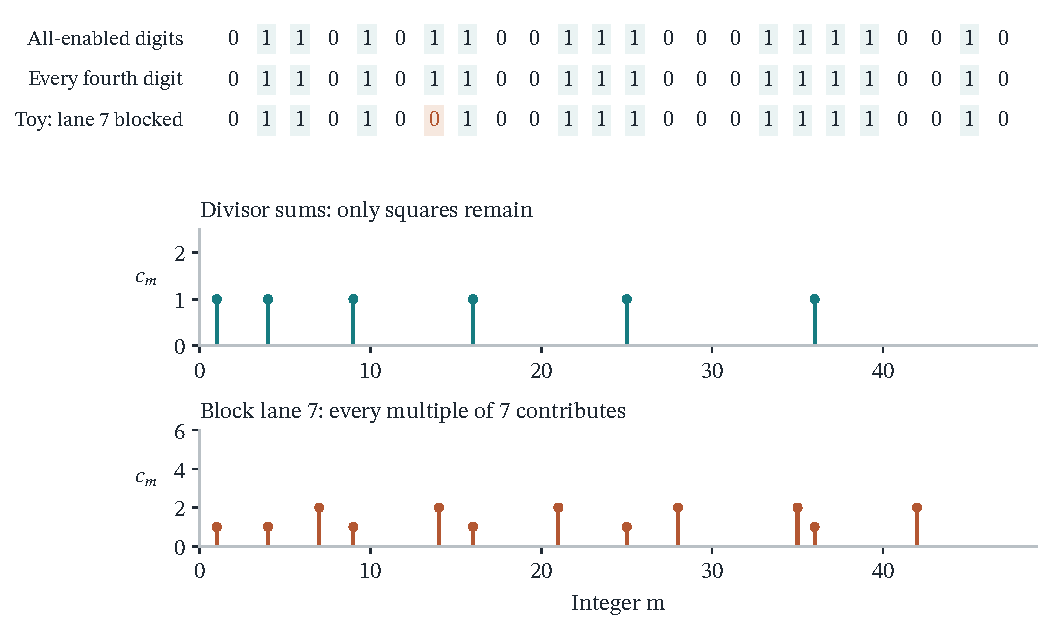
\includegraphics[width=.96\linewidth]{figures/01_digits_and_divisors.pdf}
\caption{Exact finite digit and divisor readings. The all-enabled mask is compared with an artificial mask that disables the lane of 7. The actual Goldbach question assigned to that lane is already settled by $10=5+5$. The lower plot illustrates how a failed lane would add a harmonic subseries.}
\label{fig:divisors}
\end{figure}

\subsection{A dimension change and a broken symmetry}

Exponentially damping the same divisor sums gives, for $t>0$,
\begin{equation}
 \Theta_{\Gold}(t)=1+2\sum_{m\ge1}c_me^{-\pi mt}
 =\theta(t)+4\sum_{n\ge1}\frac{b_n}{e^{\pi nt}-1},
 \qquad
 \theta(t)=\sum_{k\in\mathbb Z}e^{-\pi k^2t}.
 \label{fnd:heat-decomposition}
\end{equation}
Absolute convergence follows, for example, from
$0\le c_m\le\sum_{d\mid m}1$; the second equality follows by
summing over multiples.  It is legitimate to view $\Theta_{\Gold}$ as
the heat trace of a diagonal operator: there is one zero state and
energy $\pi m$ has multiplicity $2c_m$ whenever $c_m>0$.

\begin{proposition}[Heat-growth dimension]\label{fnd:dimension}
The limit
\[
 d_{\Gold}=2\lim_{t\downarrow0}\frac{\log\Theta_{\Gold}(t)}{\log(1/t)}
\]
exists, and equals one if Goldbach holds and two otherwise.
More precisely, in the latter case,
\begin{equation}
 \Theta_{\Gold}(t)\sim\frac{2S_g}{\pi t}\log\frac1t.
 \label{fnd:heat-leading}
\end{equation}
\end{proposition}
\begin{proof}
Under Goldbach, $\Theta_{\Gold}=\theta$, and Jacobi's transformation
$\theta(t)=t^{-1/2}\theta(1/t)$ gives
$\theta(t)\sim t^{-1/2}$; see \cite[20.7.32]{fndDLMF}.
If a lane $p$ fails, its single term in
\eqref{fnd:heat-decomposition} gives a lower bound of order
$t^{-1}$.  Since $b_n\le1$, splitting the remaining sum at
$n=1/t$ gives an upper bound $O(t^{-1}\log(1/t))$.
These estimates prove the dimension dichotomy without a density
theorem.

For the sharper equivalent, Theorem~\ref{fnd:balance} applied
lane by lane gives $\sum_{n\le y}b_n=(S_g/2)y+o(y)$.
Partial summation yields
$\sum_{n\le y}b_n/n=(S_g/2)\log y+o(\log y)$.
Consequently
\[
 \sum_{m\le y}c_m=\lfloor\sqrt y\rfloor+
 2\sum_{n\le y}b_n\lfloor y/n\rfloor
 \sim S_gy\log y,
\]
the floor error being $O(y)$.  Integrating this counting function
against $\pi t e^{-\pi ty}$ proves \eqref{fnd:heat-leading}.
Domination follows from $\sum_{m\le y}c_m=O(y\log(y+2))$.
\end{proof}

The word dimension here means the heat-growth exponent just defined.
Under Goldbach the operator agrees with the Laplacian spectrum of a
circle of circumference $2\sqrt\pi$.  The extra logarithm in
\eqref{fnd:heat-leading} is retained explicitly; no ordinary smooth
two-dimensional surface is being asserted in the other case.

\begin{proposition}[A single inversion identity]\label{fnd:inversion}
For every fixed $t>1$,
\[
 t^{-1/2}\Theta_{\Gold}(1/t)-\Theta_{\Gold}(t)\ge0,
\]
and equality holds if and only if Goldbach holds.
\end{proposition}
\begin{proof}
Jacobi's identity cancels the two theta terms in
\eqref{fnd:heat-decomposition}.  What remains is
\[
 4\sum_{n\ge1}b_n\left[
 \frac{t^{-1/2}}{e^{\pi n/t}-1}
 -\frac1{e^{\pi nt}-1}\right].
\]
Every bracket is positive.  In fact, for $u=\pi n/t$,
convexity gives $e^{t^2u}-1\ge t^2(e^u-1)$, while
$t^{-1/2}>t^{-2}$.  Thus equality forces all $b_n$ to vanish;
a failed prime lane would have $b_p=1$.
\end{proof}

The same transform can locate the first failure, if one exists.
Put $E_{\Gold}(t)=\Theta_{\Gold}(t)-\theta(t)$.  If $p_*$ is the smallest
failed-lane prime, its first nonzero exponential coefficient is four:
\begin{equation}
 E_{\Gold}(t)=4e^{-\pi p_*t}\bigl(1+O(e^{-\pi t})\bigr)
 \quad(t\to\infty),\qquad
 p_*=-\frac1\pi\lim_{t\to\infty}\frac{\log E_{\Gold}(t)}t.
 \label{fnd:first-heat-failure}
\end{equation}
To justify the error, divide the series in
\eqref{fnd:positive-divisors} by its first exponential term and
bound its remaining coefficients by the divisor function.  The
resulting tail is $O(e^{-\pi t})$ for $t\ge1$.
Moreover $-E_{\Gold}'(t)/E_{\Gold}(t)$ decreases to $\pi p_*$: its derivative
is minus the variance of the energies under their exponentially
weighted positive coefficients.  There are at least two energies,
$\pi p_*$ and $2\pi p_*$, so the decrease is strict.

\subsection{A finite exception list in a heat coefficient}

If there are finitely many disabled lanes, a further exact reading
is available.  Let $F=\{j:g_j=0\}$ be finite, and set
\[
 A(s)=\sum_{j\in F}p_j^{-s}\prod_{r<j}(1-p_r^{-s}),\qquad
 C(s)=\sum_{j\in F}p_j^{-s}\prod_{r<j}(1+p_r^{-s}),\qquad
 B=\sum_{j\in F}2^{j-1}.
\]
Here $B$ is the integer whose binary digits list the disabled lanes.
These are finite Dirichlet polynomials, and $A(1)=S_g$.

\begin{proposition}\label{fnd:heat-binary}
For a finite failed-lane set in the Goldbach construction,
\begin{align}
 \Theta_{\Gold}(t)={}&\frac2{\pi t}
 \left[S_g\log(1/t)+(\gamma-\log\pi)S_g+A'(1)\right]
 \notag\\
 &+\frac{1+C(1/2)}{\sqrt t}-B+O_F(\sqrt t)
 \qquad(t\downarrow0).
 \label{fnd:heat-binary-expansion}
\end{align}
Thus the constant term after the three divergent terms have been
removed records the entire finite exception list in binary.
\end{proposition}
The mechanism is a residue calculation: the growing terms come from the
poles at 1 and $1/2$, while the constant term comes from the pole of the
gamma factor at zero. The cancellation at that last pole leaves a sum of
distinct powers of two. The full calculation is in
Appendix~\ref{app:fnd:heat-binary}.

For example, an artificial message that disables lanes with indices
$2$ and $4$ has remaining constant term $-(2+8)=-10$. Read the magnitude
as binary $1010$: the two ones recover those exact indices. The actual
Goldbach questions attached to these lanes, $6$ and $10$, have known
representations; the example illustrates the encoding for a general mask.
The limiting growth detects that something was removed. Its finite part
can remember exactly what was removed.

The finiteness hypothesis belongs to this last proposition.  The
Basel alternative, the dimension dichotomy, and the first-failure
reading required no such assumption.  Each was obtained from the
same nonnegative divisor sums, so a single construction supplies
several different levels of information.

\IfFileExists{sections/sampling.tex}{\section{A staircase made by sampling the digits}
\label{samp:section}

Reading the digits at equally spaced positions gives another real number:
\[
 Y_g(a,d)=\sum_{j\ge0}x_g(a+jd)2^{-j-1}.
\]
Now choose the starting point $a$ and the step $d$ uniformly from
$1,\ldots,N$, subject to $\gcd(a,d)=1$.  This last restriction prevents
the entire progression from being trapped in a common prime lane.
Let $\nu_{g,N}$ be the distribution of $Y_g(a,d)$.  Its limiting
distribution gives a curve that rises across every interval, even in
examples where its derivative is zero almost everywhere.  The apparent
contradiction disappears once we distinguish total rise from the slope
at a typical point.

Write $\mathcal F=\{p_j:g_j=0\}$ for the disabled primes.  The hypothesis
needed below says that the successful primes retain a divergent
reciprocal sum:
\begin{equation}
 \sum_{p\notin\mathcal F}\frac1p=\infty.
 \label{samp:success-hypothesis}
\end{equation}
It holds unconditionally for the actual Goldbach mask.  Indeed, let
$E(Y)$ count even Goldbach exceptions in $[4,Y]$ and let
$A(R)=\#(\mathcal F\cap[2,R])$.  Pintz's Theorem~1
\cite{sampPintz2018} states that $E(Y)<Y^{18/25}$ beyond an
ineffective threshold.  The prime number theorem therefore gives
\begin{equation}
 A(R)=E\bigl(2(\pi(R)+1)\bigr)
 \ll (R/\log R)^{18/25} \quad(R\ge3).
 \label{samp:pintz}
\end{equation}
Partial summation shows $\sum_{p\in\mathcal F}1/p<\infty$, whereas
the sum over all primes diverges.  We use this established estimate
as an input.  Its precise exponent is useful later; here any power
strictly smaller than one would suffice.

\begin{theorem}[Primitive sampling]\label{samp:staircase}
Assume \eqref{samp:success-hypothesis}.  Then $\nu_{g,N}$ converges
weakly to a nonatomic probability measure $\nu_g$ of full support
$[0,1]$ and Hausdorff dimension one.  Its Lebesgue decomposition is
\begin{equation}
 \nu_g=L_g\,\mathrm{Leb}+\nu_{g,\mathrm{sc}},\qquad
 L_g=\prod_{p\in\mathcal F}\frac1{p+1},
 \label{samp:decomposition}
\end{equation}
where $\nu_{g,\mathrm{sc}}$ is singular continuous.  The empty product
is one; an infinite product here is zero.  Consequently
\[
 G_g(y):=\nu_g([0,y])\quad(0\le y\le1)
\]
is a homeomorphism of $[0,1]$ onto itself and
$G_g'(y)=L_g$ for Lebesgue-almost every $y$.
\end{theorem}

Full support means that every nonempty open interval receives positive
probability.  Singular means that a set of ordinary length zero carries
the measure.  Dimension one means that every set carrying its full mass
has Hausdorff dimension one.  These properties can coexist: small in
length need not mean small in dimension.  We do not claim that the
measure has the same local dimension at almost every point.

The mechanism is easier to see than the full convergence proof.
Choose, independently at every prime $p$, a residue pair $(U,V)\bmod p$
uniformly among the $p^2-1$ pairs other than $(0,0)$.  These simultaneous
residues are a primitive profinite pair.  Independently choose fair
bits $B_0,B_1,\ldots$.  The limiting sampled real has the law of
\[
 Z_g=\sum_{j\ge0}\bigl(1-h_g(U+jV)\bigr)B_j2^{-j-1}.
\]
Thus an open lane contributes a fair bit and a disabled lane contributes
zero.  This is a theorem about the average over starting points and
steps; it does not assume that the original consecutive digits are
independent.

A lane $p$ is visited precisely when $p$ does not divide $V$.  The
probability that it is avoided is $1/(p+1)$.  Consequently every bit is
free precisely on an event of probability $L_g$; that event supplies the
uniform part of the measure.  Once a disabled lane is visited, zeros
repeat on an infinite arithmetic progression.  Such digit strings form
a single Lebesgue-null set, which carries the remaining part.

This explains the decomposition and its product formula.  Full support
comes from making any finite prefix open by finitely many compatible
congruences.  Full dimension requires an additional limiting argument:
there are positive portions of the law with a proportion of free bits
arbitrarily close to one.  The complete proof, including the
Frantzikinakis--Host variable-step cancellation that produces the fair
bits, is in Appendix~\ref{samp:proofs}.


\begin{corollary}\label{samp:goldbach-trichotomy}
For the original Goldbach constant, $G_{\Gold}$ is the identity if and
only if Goldbach holds.  If there are finitely many exceptions and at least one, then
\[
 G_{\Gold}'(y)=\frac1{\prod_{p\in\mathcal F}(p+1)}\in(0,1)
 \quad\hbox{almost everywhere}.
\]
There are infinitely many Goldbach exceptions if and only if
$G_{\Gold}'=0$ almost everywhere.  In this last case $G_{\Gold}$ is a singular
homeomorphism whose associated measure has dimension one.
\end{corollary}

This phenomenon also has an unconditional explicit example.  Disable
exactly the lanes
\begin{equation}
 \mathcal F_* =\{p_{2^j}:j\ge2\}.
 \label{samp:explicit-mask}
\end{equation}
This is a concrete mask, defined without asking any unresolved arithmetic
question.  Its disabled-prime reciprocal sum converges because $p_{2^j}>2^j$.  The associated
$G_*$ is therefore a strictly increasing singular homeomorphism,
with full-support measure of dimension one.  Thus the geometry
exists independently of which Goldbach alternatives occur.
}{}

\section{Reading several digits at coprime positions}
\label{fnd:correlations}

The divisor reading led to a positive spectrum.  We now try a different
experiment: select several digit positions, insisting that no two have
a common prime factor.  This prevents two positions from drawing their
least prime from the same lane.  Consequently a correlation of $k$
digits can ask whether there are at least $k$ disabled lanes.

For independent uniform integers $n_1,\ldots,n_k$ in $[1,N]$, let
$\mathcal C_{k,N}$ be the event that they are pairwise coprime.
Define $M_0(g)=1$ and, for $k\ge1$,
\begin{equation}
 M_k(g)=\lim_{N\to\infty}
 \E\left[\prod_{i=1}^k a_g(n_i)\,\middle|\,\mathcal C_{k,N}\right].
 \label{fnd:marked-moments}
\end{equation}
We will prove that this limit exists.  Throughout this section an
arbitrary binary mask is allowed, including $g_1=0$.

At one prime $p$, pairwise coprimality permits either no divisible
coordinate or exactly one.  Their total probability is
$(1-1/p)^k+k p^{-1}(1-1/p)^{k-1}$.  It follows that
\begin{equation}
 K(k)=\lim_{N\to\infty}\Prob(\mathcal C_{k,N})
 =\prod_p(1-p^{-1})^k\left(1+\frac{k}{p-1}\right)>0.
 \label{fnd:coprime-kernel}
\end{equation}
To justify the infinite product, first impose the restrictions only at
primes at most $R$ and use the Chinese remainder theorem.  The probability
of a collision at a larger prime is at most
$\binom{k}{2}\sum_{p>R}p^{-2}$, uniformly in $N$.
This tends to zero, and the local factors differ from one by
$O_k(p^{-2})$.  In particular $K(0)=K(1)=1$ and
$K(2)=1/\zeta(2)=6/\pi^2$.

The Euler product in \eqref{fnd:coprime-kernel} is classical.  Written
as
$\prod_p(1-1/p)^{s-1}(1+(s-1)/p)$, it is the arithmetic factor
appearing in mod-Poisson descriptions of the number of distinct prime
divisors; see \cite[Section 4]{fndKowalskiNikeghbali2009}.
Here its role is dictated by the coprimality experiment itself.

\begin{proposition}[Correlations count available lanes]
\label{fnd:moment-positivity}
The limits in \eqref{fnd:marked-moments} exist and satisfy
\begin{equation}
 0\le M_k(g)\le1,\qquad M_1(g)=S_g,\qquad
 M_k(g)>0\ \Longleftrightarrow\ \#\{j:g_j=0\}\ge k.
 \label{fnd:moment-tests}
\end{equation}
They have the following probability description.  Independently at
each prime $p$, choose one of $k$ coordinates with probability
$1/(p+k-1)$ each, or choose none with probability
$(p-1)/(p+k-1)$.  A coordinate is labelled by the first prime that
chooses it.  Then $M_k(g)$ is the probability that all $k$ labels
belong to disabled lanes.
\end{proposition}
Each factor $a_g(n_i)$ is a sign, so its product can be negative.
Yet the limit is a probability. Averaging cancels the Liouville oscillation
on every enabled lane; the disabled lanes leave a persistent contribution.
Coprimality forces the first prime labels to be distinct. Those two facts
explain both the nonnegativity and the exact counting test. The truncation
argument that justifies them is in Appendix~\ref{app:correlations}.


We collect the correlations into two entire functions,
\begin{equation}
 \Phi_g(z)=\sum_{k\ge0}M_k(g)\frac{z^k}{k!},\qquad
 \Psi_g(z)=\sum_{k\ge0}K(k)M_k(g)\frac{z^k}{k!}.
 \label{fnd:two-functions}
\end{equation}
Both series converge absolutely everywhere, with modulus at most
$e^{|z|}$.  The first averages after conditioning on coprimality;
the second gives noncoprime tuples score zero and averages over
all tuples.  If there are exactly $r$ disabled lanes, each function
is a polynomial of degree $r$.  Under Goldbach both are identically
one.  When there are infinitely many disabled lanes, every
coefficient is positive.

\subsection{A positive operator behind the correlations}

The change from conditional to unconditional averages has a strong
spectral effect.  Its proof also gives an explicit construction.
A positive operator is a matrix with a nonnegative quadratic form,
possibly on an infinite-dimensional space. Its eigenvalues are nonnegative.
In the theorem below they also have a finite sum. Such an operator has a
determinant $\prod_j(1+\alpha_j z)$, so its zeros can lie only on the
negative real axis. The assertion is that the unconditional correlation
function has precisely this structure. Write $\mathcal F=\{p_j:g_j=0\}$
for its disabled primes.

\begin{theorem}[The positive mask operator]\label{fnd:mask-operator}
For every prime mask there is a positive trace-class operator $A_g$
with
\begin{equation}
 \Psi_g(z)=\det(I+zA_g),\qquad
 \operatorname{tr}A_g=S_g,\qquad
 \operatorname{rank}A_g=\#\mathcal F.
 \label{fnd:positive-determinant}
\end{equation}
The rank may be infinite.  Every zero of $\Psi_g$ is negative and real.
\end{theorem}
The construction processes primes one at a time. Each disabled lane
adds one positive spectral direction, while the trace records the total
disabled-lane density. Appendix~\ref{app:fnd:mask-operator} gives the
explicit differential recurrence and the limiting operator.

This explains the rank statement in ordinary terms: counting the
operator's nonzero directions counts the missing answers. If exactly
three lanes are disabled, the infinite construction produces only three
such directions.

The proof establishes a summable spectrum for every mask, without
requiring any estimate for Goldbach's exceptional set.  It also gives
the useful bound
\begin{equation}
 K(k)M_k(g)\le S_g^k.
 \label{fnd:moment-bound}
\end{equation}
Indeed, $K(k)M_k(g)/k!$ is the $k$th elementary symmetric function
of the $\alpha_j$, and the distinct-index terms in
$(\sum_j\alpha_j)^k$ contribute exactly $K(k)M_k(g)$.

\subsection{Two missing lanes, two geometries of zeros}

The distinction between the two correlation functions becomes visible
in a small example. Artificially disable just the lanes of $3$ and $5$.
Their densities add to $1/6+1/15=7/30$. Two coprime positions can use
those two lanes in either order; the prime-assignment model gives
$M_2=2(1/3)(1/4)(1/6)=1/36$. Consequently
\[
 \Phi_g(z)=1+\frac7{30}z+\frac1{72}z^2,
 \qquad
 \Psi_g(z)=1+\frac7{30}z+\frac1{12\pi^2}z^2.
\]
The discriminant of the first polynomial is $-1/900$, so its two zeros
are nonreal. The second has two negative real zeros, as the operator
theorem requires. The same two disabled lanes have produced both
geometries. Conditioning on coprimality changes the zeros, even though
both functions retain the exact count of missing lanes.

\begin{figure}[htbp]
\centering
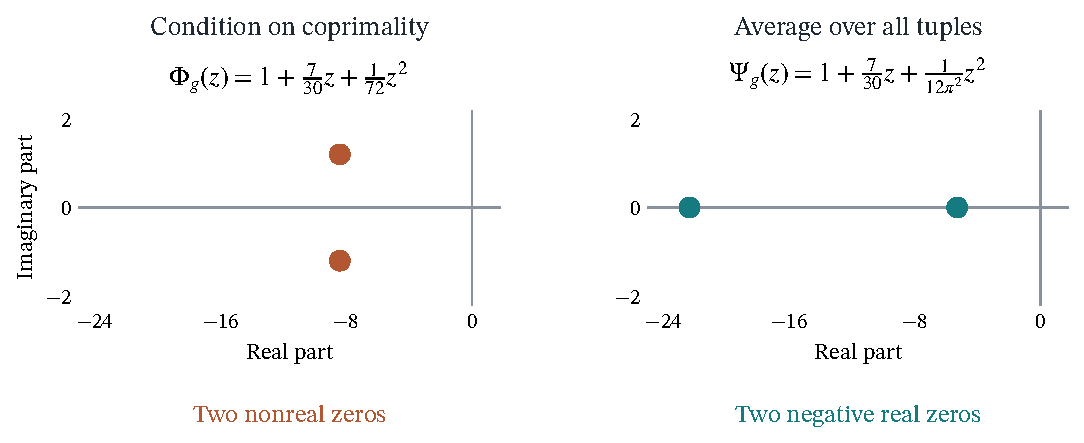
\includegraphics[width=.96\linewidth]{figures/05_two_averages.pdf}
\caption{The same artificial message disables the lanes of 3 and 5.
Conditioned and unconditioned correlations give two quadratic polynomials
with different zero locations. The coefficients are exact; coordinates
in the plot are their numerical root locations.}
\label{fig:two-averages}
\end{figure}

This is the question that will lead to the curve: can we describe that
change of average by introducing an independent random scale?

\IfFileExists{sections/phi_growth.tex}{\subsection{What the growth and zeros count}
\label{grw:section}

The operator behind $\Psi_g$ controls the location of its zeros.
The companion $\Phi_g$ records how quickly disabled lanes accumulate.
If those primes grow sparse, the function grows slowly; if they grow
more numerous, it grows faster.  For the Goldbach member this comparison
also turns the conjecture into a statement about complex zeros.

Put $a_k=M_k(g)/k!$ and $B_g(R)=\#(\mathcal F\cap[2,R])$.
If all $k$ labels in the prime-assignment model of
Proposition~\ref{fnd:moment-positivity} are masked, their first
assigned primes are $k$ distinct members of $\mathcal F$.
For a chosen set of $k$ primes, sum over its $k!$ assignments to the
labels and discard the first-assignment restrictions.  Independence
between primes gives the useful bound
\begin{equation}
 a_k\le e_k\left(\frac1{p+k-1}:p\in\mathcal F\right)
 \le e_k\left(\frac1p:p\in\mathcal F\right),
 \label{grw:coefficient-majorant}
\end{equation}
Here $e_k$ means the sum of products over all $k$-element subsets; for
example $e_2(w)=\sum_{p<q}w_pw_q$.  Thus, when
$\sum_{p\in\mathcal F}1/p<\infty$,
\begin{equation}
 |\Phi_g(z)|\le\Phi_g(|z|)
 \le P_{\mathcal F}(|z|):=
       \prod_{p\in\mathcal F}(1+|z|/p).
 \label{grw:majorant}
\end{equation}
The product bounds the function from above.  Its factors are not being
identified with the zeros of $\Phi_g$.

The \emph{order} of an entire function records the power in its
exponential growth: roughly, growth like $\exp(r^\alpha)$ on disks of
radius $r$ gives order $\alpha$.  The following theorem matches that
analytic exponent with a counting exponent for the disabled primes.

\begin{theorem}[Counting exponent and entire-function order]
\label{grw:order}
Suppose the disabled-prime counting exponent
\[
 \eta_g=\limsup_{R\to\infty}
 \frac{\log\max(1,B_g(R))}{\log R}
\]
is strictly less than one.  Then $\Phi_g$ has order exactly $\eta_g$.
Formally the order is the limsup of $\log\log \max_{|z|\le r}|\Phi_g(z)|$
divided by $\log r$; constants and polynomials have order zero by convention.  For the actual
Goldbach mask,
\begin{equation}
 \operatorname{ord}\Phi_{\Gold}
 =\limsup_{Y\to\infty}\frac{\log\max(1,E(Y))}{\log Y}
 \le\frac{18}{25},
 \label{grw:goldbach-order}
\end{equation}
and, as $r\to\infty$,
\begin{equation}
 \log\max_{|z|\le r}|\Phi_{\Gold}(z)|
 =\log\Phi_{\Gold}(r)\ll(r/\log r)^{18/25}.
 \label{grw:quantitative-growth}
\end{equation}
In particular, for an absolute constant $C$ and $k\ge2$,
\begin{equation}
 M_k(\Gold)\le
 \left(\frac{C}{k^{7/18}\log(k+1)}\right)^k.
 \label{grw:moment-bound}
\end{equation}
\end{theorem}
The proof is in Appendix~\ref{grw:proofs}.  Its two estimates have
opposite roles.  Summing over every possible set of disabled primes
bounds the function from above.  Requiring the first $k$ disabled
primes to hit distinct labels supplies a matching lower bound on its
order.  The analytic exponent therefore cannot lose the arithmetic
counting exponent.


\begin{corollary}[Zeros count the exceptions]\label{grw:zeros}
Under the hypothesis of Theorem~\ref{grw:order}, list the zeros
of $\Phi_g$ with multiplicity as $(\zeta_j)$.  Then
\begin{equation}
 \Phi_g(z)=\prod_j(1-z/\zeta_j),\qquad
 \sum_j|\zeta_j|^{-1}<\infty,\qquad
 \sum_j\zeta_j^{-1}=-S_g.
 \label{grw:factorization}
\end{equation}
Counting multiplicity, the number of zeros equals the number of
disabled lanes, allowing infinity.
If $n_g(R)$ counts the zeros in $|z|\le R$, with multiplicity, then
\begin{equation}
 \limsup_{R\to\infty}
 \frac{\log\max(1,n_g(R))}{\log R}=\eta_g.
 \label{grw:zero-exponent}
\end{equation}
For the actual Goldbach function,
\[
 \GC\ \Longleftrightarrow\ \Phi_{\Gold}\text{ has no complex zeros},
 \qquad n_{\Gold}(R)\ll(R/\log R)^{18/25}.
\]
If there are infinitely many exceptions, every complex value is
attained by $\Phi_{\Gold}$ infinitely often.
\end{corollary}
\begin{proof}
Hadamard's factorization theorem \cite{sampHadamard1893} says that
an entire function of order less than one has a genus-zero product
and a constant exponential prefactor.  Since $\Phi_g(0)=1$, this
gives the first two assertions of \eqref{grw:factorization};
differentiation at zero gives its last assertion because
$\Phi_g'(0)=M_1(g)=S_g$.  For a finite mask the polynomial degree
is $\#\mathcal F$.  For an infinite mask all coefficients are
positive, so the function is not a polynomial; the factorization
then forces infinitely many zeros.  The same argument applied to
$\Phi_g-w$ shows infinite attainment of each $w\in\mathbb C$
when the mask is infinite.

Jensen's formula and $\Phi_g(0)=1$ give
$n_g(R)\log2\le\log\Phi_g(2R)$, which bounds the zero-counting
exponent by $\eta_g$ and gives the displayed quantitative estimate.
Conversely, if that exponent were $\lambda<\eta_g$, choose
$\lambda<\beta<\eta_g<1$.  The product
\eqref{grw:factorization}, together with
$n_g(t)\ll_\beta t^\beta$, implies
\[
 \log\max_{|z|\le r}|\Phi_g(z)|
 \le\sum_j\log(1+r/|\zeta_j|)=O_\beta(r^\beta)
\]
by the same integration used in \eqref{grw:stieltjes}, starting
below the smallest zero modulus.  This contradicts its order.
The zero-order case follows from the upper bound and nonnegativity.
\end{proof}

These are zeros of the mask function.  The worked example above shows
that they can be nonreal.  The sparsity hypothesis is essential to the
factorization argument.
Also, order zero alone does not mean finitely many exceptions: an
infinite mask with subpower counting function has the same order.
The improved moment estimate measures a statistic of our
construction; it does not improve the imported bound for $E(Y)$.

\subsection{One bias can hide infinitely many changes}
\label{grw:collision-section}

There is a sharp reason to keep the higher correlations rather
than only the proportion of zero digits.  Put
$\delta_p=p^{-1}\prod_{q<p}(1-1/q)$, so
$S_g=\sum_{p\in\mathcal F}\delta_p$.

\begin{proposition}\label{grw:bias-collision}
Among masks known to have finitely many disabled lanes, the exact bias $S_g$ determines the mask.
Nevertheless, for every sufficiently large prime $p$, there is an
infinite set $\mathcal H=\{q_1<q_2<\cdots\}$ of primes greater than
$p$ such that
\begin{equation}
 \sum_{q\in\mathcal H}\delta_q=\delta_p,\qquad
 q_{j+1}/q_j\longrightarrow\infty,
 \qquad \#(\mathcal H\cap[2,R])=o(\log R).
 \label{grw:collision}
\end{equation}
Thus two masks can have exactly the same digit bias while one has
one disabled lane and the other has infinitely many.
\end{proposition}
\begin{proof}
If $P$ is the largest prime of a finite nonempty mask, then
$\delta_P$ has $P$-adic valuation $-1$: its numerator contains only
factors $q-1<P$, and its denominator is the primorial through $P$.
Every earlier $\delta_q$ has nonnegative $P$-adic valuation.
Consequently $P$ is the largest prime dividing the reduced
denominator of $S_g$.  Recover $P$, subtract $\delta_P$, and repeat.

List all primes as $p_i$ and set $d_i=\delta_{p_i}$.  These weights
decrease strictly to zero and
\[
 d_i/d_{i+1}=p_{i+1}/(p_i-1)\longrightarrow1
\]
by the prime number theorem.  Choose $p$ beyond a point where every
consecutive ratio is less than two.  Starting with residual
$r_0=\delta_p$, repeatedly subtract the largest weight at a prime
greater than $p$ which does not exceed the residual.
The first choice is the successor of $p$.  If $q$ is a later
choice and $q^-$ its immediate prime predecessor, the residual
after subtraction satisfies
\[
 0\le r_{\mathrm{new}}
 \le\delta_{q^-}-\delta_q=o(\delta_q).
\]
The ratio bound makes $r_{\mathrm{new}}<\delta_q$, so no weight is
used twice and selected primes strictly increase.  The process
cannot terminate: a finite sum at primes greater than $p$ has a
reduced denominator containing its largest prime, unlike
$\delta_p$.  It therefore makes infinitely many selections, and
$r_j<\delta_{q_j}\to0$ proves the sum identity.

The next selected weight is at most the preceding residual, hence
$\delta_{q_{j+1}}/\delta_{q_j}\to0$.  Mertens' product estimate
$\delta_q\sim e^{-\gamma}/(q\log q)$ forces
$q_{j+1}/q_j\to\infty$.  For any fixed $C>1$, these ratios
eventually exceed $C$, so the counting function is at most
$\log R/\log C+O_C(1)$.  Letting $C$ tend to infinity proves
\eqref{grw:collision}.
\end{proof}

The equality is exact, so it survives arbitrarily accurate measurement
of the digit frequency.  For these two masks $\Phi_g'(0)$ agrees,
but their functions are
respectively linear and transcendental entire.  The second has
order zero and infinitely many zeros by the preceding results.
This is an example within the mask family; it asserts no actual
Goldbach exception, and no collision between the whole functions.
}{}

\section{The curve selected by coprimality}
\label{fnd:curve-section}

The positive operator belongs to a particular message.  The factor
$K(k)$ that connected its determinant with the original correlations
does not.  We now isolate that universal factor.  Define
\begin{equation}
 K(s)=\prod_p(1-p^{-1})^s\left(1+\frac{s}{p-1}\right),
 \qquad s\in\mathbb C,
 \label{fnd:entire-k}
\end{equation}
using the real logarithm of $1-1/p$.  The local factor is
$1+O_B(p^{-2})$ on $|s|\le B$, so the product is entire.
Its zeros are simple and occur precisely at $s=1-p$:
away from these points the logarithm of the tail converges
absolutely, and at each such point exactly one factor vanishes.

The reciprocals of its nonnegative integer values are moments of a
positive random variable.  This kind of reciprocal-Mellin construction,
including its role in cancelling arithmetic factors by an auxiliary
random scale, occurs in Barhoumi--Andr\'eani's dissertation
\cite[Section 3.6.1]{fndBarhoumi2013}.  Its general mechanism is
therefore prior work.  Our aim here is the concrete coprimality law
and its actual density.

\begin{proposition}[The universal scale]\label{fnd:prime-noise}
Let $(U_p)_p$ be independent uniform variables on $(0,1)$.  The product
\begin{equation}
 W=\prod_p\frac p{p-1}U_p^{1/(p-1)}
 \label{fnd:w-product}
\end{equation}
converges almost surely to a finite positive random variable, and
\begin{equation}
 \E W^s=\frac1{K(s)}\qquad(\Re s>-1).
 \label{fnd:mellin}
\end{equation}
This is the exact half-plane of finite absolute moments.  In particular,
$\E W=1$ and $\Var W=\pi^2/6-1$.
\end{proposition}
\begin{proof}
Write $E_p=-\log U_p$, so the $E_p$ are independent exponentials
of mean one.  The logarithm of the $p$th factor is
$\log(p/(p-1))-E_p/(p-1)$.  Its mean is $O(p^{-2})$
and its variance is $(p-1)^{-2}$.  The centered independent series
converges almost surely and in $L^2$, while its means sum absolutely.
Exponentiation proves the product assertion.

For a finite prime cutoff $R$, direct integration gives
$\E W_R^s=1/K_R(s)$ for $\Re s>-1$.  If $\sigma=\Re s$,
choose $r>1$ with $r\sigma>-1$; this is always possible.
The product of moments $\E W_R^{r\sigma}$ is uniformly bounded,
since its local factors are $1+O_{s,r}(p^{-2})$.
Thus $(W_R^s)_R$ is uniformly integrable, and almost-sure
convergence proves \eqref{fnd:mellin}.
For $\sigma\le-1$, write $W=2U_2V$ with $V>0$ independent
of $U_2$.  Conditional integration over $U_2$ makes
$\E W^\sigma$ infinite.  Finally $K(1)=1$ and
$K(2)=6/\pi^2$ give the stated mean and variance.
\end{proof}

In terms of the cited general construction, the logarithm of $W$ is
a deterministic constant plus
$\sum_p (1-E_p)/(p-1)$.  This identifies the specialization directly.
The same scale now reverses the coprimality weighting of every message.

\begin{corollary}[The exact bridge]\label{fnd:bridge}
For every mask and every $z\in\mathbb C$,
\begin{equation}
 \Phi_g(z)=\E\Psi_g(zW)=\E\det(I+zWA_g).
 \label{fnd:bridge-equation}
\end{equation}
\end{corollary}
\begin{proof}
All coefficients of $\Psi_g$ are nonnegative.  Tonelli and
\eqref{fnd:mellin} give
\[
 \E\Psi_g(|z|W)=
 \sum_{k\ge0}K(k)M_k(g)\frac{|z|^k}{k!}\E W^k
 =\Phi_g(|z|)\le e^{|z|}.
\]
Absolute integrability therefore permits the same termwise exchange
for complex $z$, proving the identity.
\end{proof}

We have reached a division of roles.  The operator carries the
message; $W$ carries the universal effect of changing the average.
It is this universal law that produces the curve in the title.

\subsection{The entire density theorem}

A probability density is initially a real function, defined on the
possible values of its random variable.  The density here has an
additional analytic structure: it continues to an entire function,
and the positions of its nonzero Taylor coefficients recover the
primes exactly.  Reciprocal transforms of real-zero entire products
have a classical theory, notably Schoenberg's
\cite{fndSchoenberg1947}; the following proof establishes this
specific density and the required convergence directly.

\begin{theorem}[The prime density]\label{fnd:entire-density}
The random variable $W$ has a density on $(0,\infty)$ which extends
to the entire function
\begin{equation}
 f(z)=\sum_{p\text{ prime}}\frac{z^{p-2}}{K'(1-p)}.
 \label{fnd:density-series}
\end{equation}
Consequently
\begin{equation}
 f^{(n)}(0)\ne0\quad\Longleftrightarrow\quad n+2\text{ is prime}.
 \label{fnd:prime-taylor-support}
\end{equation}
With $c_p=1/K'(1-p)$, the nonzero coefficients have signs
$\operatorname{sgn}(c_p)=(-1)^{\pi(p)-1}$ and satisfy
\begin{equation}
 \log|c_p|=-p\log\log p+O(p).
 \label{fnd:residue-decay}
\end{equation}
\end{theorem}

\paragraph{Why a probability density contains this pattern.}
With only finitely many primes, take logarithms of the defining random
product. We obtain a sum of independent exponential variables, whose
rates are $p-1$. Returning from logarithms turns these rates into powers
$z^{p-2}$ in a finite density formula. As the prime cutoff grows, the
right endpoint of that formula moves to infinity and its coefficients
converge. This is how the primes become derivative positions.

There are two things to prove: convergence of the entire series, and
identification of its restriction to the positive axis with the actual
probability density. Appendix~\ref{app:fnd:entire-density} proves both,
including the coefficient estimate in the theorem.

The support of the Taylor series begins
\[
 f(z)=c_2+c_3z+c_5z^3+c_7z^5+c_{11}z^9+c_{13}z^{11}+\cdots.
\]
The construction did not begin by writing down a prime-supported
series.  It began with coprimality probabilities, then produced a
positive random scale and finally its density.  The theorem says
that positivity, normalization, entire continuation and this exact
prime pattern coexist in the same curve.

Consider what the derivative test says at its first few positions.
The second derivative vanishes at zero because $2+2=4$ is composite.
The third derivative does not vanish because $3+2=5$ is prime. The
fourth vanishes, and the fifth does not. The test continues forever.
These are exact zeros amid exact nonzeros, rather than a tendency for
prime positions to have larger coefficients.

The source of the curve is equally important. An observer can describe
the sampling experiment and ask for the resulting probability density
before asking any question about its derivatives. The arithmetic pattern
then appears inside that density. This is what distinguishes the result
from merely choosing a list of coefficients indexed by primes.

\begin{figure}[htbp]
\centering
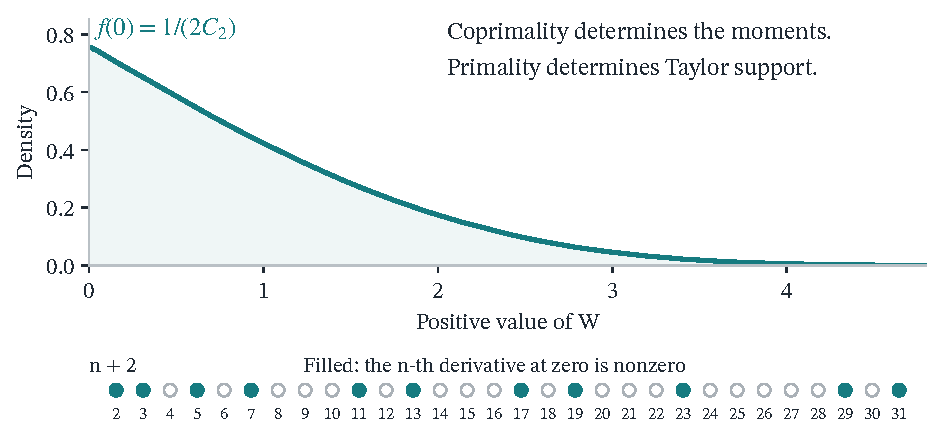
\includegraphics[width=.96\linewidth]{figures/02_prime_density.pdf}
\caption{The density on the positive axis and its exact Taylor-support pattern. The curve is an explicitly approximate conditional Monte Carlo preview with 180,000 samples, primes through 2,000 and seed 271828; no numerical error certificate is claimed. The marked derivative positions represent Theorem~\ref{fnd:entire-density}, not a numerical derivative test.}
\label{fig:density}
\end{figure}

\subsection{Reflection, a symmetric distribution, and the twin constant}

Let
\begin{equation}
 \mathfrak C_2=\prod_{p>2}\frac{p(p-2)}{(p-1)^2}
 \label{fnd:twin-constant}
\end{equation}
be the usual twin-prime constant.  Its appearance below uses only
this convergent product, with no assertion about twin-prime
infinitude.

\begin{corollary}\label{fnd:reflection}
The entire density satisfies
\begin{equation}
 f(0)=\frac1{2\mathfrak C_2},\qquad
 f(z)+f(-z)=\frac1{\mathfrak C_2}\quad(z\in\mathbb C).
 \label{fnd:reflection-identity}
\end{equation}
It is nonincreasing on the real line, with limits
$1/\mathfrak C_2$ and zero at negative and positive infinity,
respectively.  Consequently
\[
 \SymCDF(x)=\mathfrak C_2 f(-x)
\]
is a symmetric cumulative distribution function on $\mathbb R$.
The entire function $f$ is bounded on the real axis and has
infinite order in the complex plane.
\end{corollary}
\begin{proof}
Writing $W=2U_2V$ and conditioning on $V$ gives
\begin{equation}
 f(w)=\E\left[\frac1{2V}\mathbf1_{\{2V>w\}}\right],
 \qquad w>0.
 \label{fnd:density-monotone}
\end{equation}
The independent prime-$3$ factor makes the distribution of $V$
nonatomic.  Once its inverse moment below is finite, dominated
convergence makes the right-hand side continuous, so this identity
holds pointwise for the entire density, not merely almost everywhere.
The inverse moment of $V$ is
$\E V^{-1}=\prod_{p>2}(p-1)^2/[p(p-2)]=1/\mathfrak C_2$;
the moment passage follows as in Proposition~\ref{fnd:prime-noise},
now with domain $\Re s>-2$.  Thus
$f(0)=1/(2\mathfrak C_2)$ and $f$ is nonincreasing on the
positive half-line.  Integrability makes its limit there zero.
Every nonconstant exponent $p-2$ in
\eqref{fnd:density-series} is odd, proving the reflection identity.
This extends the monotonicity and gives the two endpoint limits,
from which the CDF assertion follows.

For completeness, the coefficient formula for the order of an
entire series is
$\rho=\limsup_{n\to\infty}n\log n/\log(1/|[z^n]f|)$,
with zero coefficients omitted.  Along $n=p-2$,
\eqref{fnd:residue-decay} makes this ratio asymptotic to
$\log p/\log\log p$, which tends to infinity.
\end{proof}

Thus a smooth bounded curve on the real line can have extremely
large growth in other complex directions.  For every fixed $a>0$, there are arbitrarily large $R$ for which
$\max_{|z|=R}|f(z)|>\exp(R^a)$, even though $f$ stays bounded on the
whole real axis. The prime pattern is
local analytic information at zero; ordinary plotting resolution
does not reveal its vanishing derivatives.  The reflection identity
provides a simple real counterpart of that analytic structure.

\subsection{Put the composites back}

The product defining $W$ uses only prime indices.  The missing
composite factors complete it to a familiar distribution.  On an
independent family of uniform variables define
\begin{equation}
 \Comp=\prod_{\substack{m\ge4\\m\text{ composite}}}
       \frac m{m-1}U_m^{1/(m-1)}.
 \label{fnd:composite-noise}
\end{equation}
Its logarithm converges by the same summable-mean and summable-variance
argument as before. We can now ask a simple question: what happens if
the prime contribution and the composite contribution are put back
together? The answer is the standard exponential distribution, whose
density is $e^{-w}$ for $w>0$.

\begin{proposition}[Prime--composite completion]\label{fnd:completion}
For independent $W$ and $\Comp$ defined above,
\begin{equation}
 W\Comp\ \overset{d}=\ \operatorname{Exp}(1),\qquad
 \E \Comp^s=\Gamma(1+s)K(s)\quad(\Re s>-1).
 \label{fnd:completion-law}
\end{equation}
\end{proposition}
\begin{proof}
Combine all integer factors up to $M$:
\[
 V_M=\prod_{m=2}^{M}\frac m{m-1}U_m^{1/(m-1)}.
\]
Its Mellin transform is
\[
 \E V_M^s=M^s\prod_{j=1}^{M-1}\frac j{j+s}
 =M^s\frac{\Gamma(M)\Gamma(1+s)}{\Gamma(M+s)}.
\]
This is also the Mellin transform of
$M\min(U_1,\ldots,U_{M-1})$, as follows directly by integrating
the density of the minimum.  Characteristic functions of the
logarithms identify the two laws.  For fixed $x\ge0$ and $M>x$,
the survival probability of the latter variable is
$(1-x/M)^{M-1}\to e^{-x}$.  Meanwhile $V_M$ converges almost
surely to the product $W\Comp$.  Thus $W\Comp$ is exponential.
Uniform integrability of fixed moments with real part greater
than $-1$ follows from a nearby moment exactly as in
Proposition~\ref{fnd:prime-noise}.  Independence and
\eqref{fnd:mellin} now give the second identity.
\end{proof}

This completion is a short specialization of classical beta and gamma
product identities.  It will also supply the composite random scale
in the later matrix construction.  The path from the constant to the
curve has therefore produced more than an encoding: the same
coprimality factor can change conditional averages, generate a
positive spectrum, and connect two complementary random products.

The second moments give a small numerical glimpse of this cancellation:
\[
 \E W^2=\frac{\pi^2}{6},\qquad
 \E \Comp^2=\frac{12}{\pi^2},\qquad
 \E(W\Comp)^2=2.
\]
The complete law, and not only this moment, becomes exponential.
The prime and composite factors separately retain their arithmetic
structure; their independent product reconstructs the distribution
obtained by allowing every integer factor.
